%% abtex2-modelo-include-comandos.tex, v-1.9.5 laurocesar
%% Copyright 2012-2015 by abnTeX2 group at http://www.abntex.net.br/ 
%%
%% This work may be distributed and/or modified under the
%% conditions of the LaTeX Project Public License, either version 1.3
%% of this license or (at your option) any later version.
%% The latest version of this license is in
%%   http://www.latex-project.org/lppl.txt
%% and version 1.3 or later is part of all distributions of LaTeX
%% version 2005/12/01 or later.
%%
%% This work has the LPPL maintenance status `maintained'.
%% 
%% The Current Maintainer of this work is the abnTeX2 team, led
%% by Lauro César Araujo. Further information are available on 
%% http://www.abntex.net.br/
%%
%% This work consists of the files abntex2-modelo-include-comandos.tex
%% and abntex2-modelo-img-marca.pdf
%%

% ---
% Este capítulo, utilizado por diferentes exemplos do abnTeX2, ilustra o uso de
% comandos do abnTeX2 e de LaTeX.
% ---
 
\chapter{Background}\label{ch:background}
% ---
\section{Similar Selection Systems}
% ---
\noindent
The system most similar to ours is RIDA$\sp{*}$ Barley et al., (\citeyear{BarleySantiagoOver}). RIDA$\sp{*}$ also selects a subset from a pool of heuristics to guide the A$\sp{*}$ search. In RIDA$\sp{*}$ this is done by starting with an empty subset and trying all combinations of size one before trying the combinations of size two and so on. RIDA$\sp{*}$ stops after evaluating a fixed number of subsets. While RIDA* is able to evaluate sets of heuristics with only tens of elements. By contrast, the method we propose in this dissertation is able to evaluate sets with thousands of elements.

Rayner et al., (\citeyear{raynersss13}) present an optimization procedure that is similar to ours. In contrast with our work, Rayner et al. limited their experiments to a single objective function that sought to maximize the sum of heuristic values in the state space. Moreover, Rayner et al.'s method performs an uniform sampling of the state space to estimate the sum of heuristic values in the state space. Thus, their method is not directly applicable to domain-independent planning. In this dissertation we adapt Rayner et al.'s approach to domain-independent planning by using Chen (\citeyear{chen1992heuristic}) Stratified Sampling to estimate the sum of heuristic values in the state space. Our empirical results show that \texttt{GHS} minimizing an approximation of A$\sp{*}$'s running time is able to substantially outperform Rayner et al.'s approach in domain-independent planning. 

Our meta-reasoning requires a prediction of the number of nodes expanded by A$\sp{*}$ using any given subset. The prediction system we choose is Stratified Sampling (\texttt{SS} system Lelis et al., (\citeyear{lelis2013predicting})). Even though, \texttt{SS} produce good predictions for Iterative Deepening$-$A$\sp{*}$, it does not give us good predictions for A$\sp{*}$ because it is unable to detect duplicated nodes during search.

% ---
\section{Problem definition}
% ---

A $SAS\sp{+} planning\ task$ B$\ddot{a}$ckstr$\ddot{o}$m; Nebel, (\citeyear{backstrom1995complexity}) is a 4 tuple $\nabla = \{V, O, I, G\}.$ \textit{V} is a set of \textit{state variables.} Each variable \textit{v} $\in$ \textit{V} is associated with a finite domain of possible $D_{\substack{v}}$. A state is an assignment of a value to every $v \in V.$ The set of possible states, denoted \textit{V}, is therefore $D_{\substack{v_{\substack{1}}}}    \times ... \times D_{\substack{v_{\substack{2}}}}$. \textit{O} is a set of operators, where each operator $o \in O$ is triple $\{pre_{\substack{o}} , post_{\substack{o}}, cost_{\substack{o}}\}$ specifying the preconditions, postconditions (effects), and non-negative cost of \textit{o}. $pre_{\substack{o}}\ and\ post_{\substack{o}}$ are assignments of values to subsets os variables, $V_{\substack{pre_{\substack{o}}}}\ and\ V_{\substack{post_{\substack{o}}}}$, respectively. Operator \textit{o} is applicable to state \textit{s} if \textit{s} and $pre_{\substack{o}}$ agree on the assignment of values to variables in $V_{\substack{pre_{\substack{o}}}}$. The effect of \textit{o}, when applied to \textit{s}, is to set the variables in $V_{\substack{post_{\substack{o}}}}$ to the values specified in $post_{\substack{o}}$ and to set all other variables to the value they have in \textit{s}. \textit{G} is the goal condition, an assignment of values to a subset of variables, $V_{\substack{G}}$. A state is a goal state if it and \textit{G} agree on the assignment of values to the variable in $V_{\substack{G}}$. \textit{I} is the initial state, and the planning task, $\nabla$, is to find an optimal (least-cost) sequence of operators leading from \textit{I} to a goal state. We denote the optimal solution cost of $\nabla$ as $C\sp{*}$. 

The state space problem illustrated in the Figure \ref{fig:8tilepuzzle_begin} consists in a board with 8 squares named tiles numbered from 1 to 8 and one square without tile and number named empty tile. The goal of the game is to order the tiles in some order. For example: From left to right and up to bottom in the following order 1, 2, 3, 4, 5, 6, 7, 8 and empty tile or ordering the tiles around the center of the board. The particular game showed is the 8-tile-puzzle, the objective of this game is to place the tiles in order by moving the numbered tiles into the empty tile. For this case, the goal would be reached by placing the tiles 1, 2 and 3 in the first row, and 4, 5 and 6 in the following row, and 7, 8 and empty tile in the last row.

\iffalse
Schaeffer; Herik, (\citeyear{Schaeffer:2002:GCA:512148.512149}) Any tile horizontally or vertically adjacent to the blank can be slid into that position. The problem is to rearrange the tiles from some random initial configuration into a particular desired goal configuration. The 8-puzzle contains 181,440 reachable states, the 15$-$puzzle contains about $10\sp{13}$ reachable states, and the 24-puzzle contains almost $10\sp{25}$ states.
\fi

\begin{figure}[htb]
\centering
\begin{forest}
 [\usebox\myboxa \hspace*{1.4in} \usebox\myboxb]
 $\node [xshift=-5.5cm,yshift=3.5cm] (A) at (2,0) {Initial};$
 $\node [xshift=1.5cm,yshift=3.5cm] (A) at (2,0) {Goal};$
\end{forest}
\caption{The left tile-puzzle is the initial distribution of tiles and the right tile-puzzle is the goal distribution of tiles. Each one represent a state.} \label{fig:8tilepuzzle_begin}
\end{figure}

Instead of using an algorithm of Brute force search that will analyze all the possible solutions, we can obtain heuristics from the problem of the sliding-tile puzzle that will help us to solve the problem.

\section{Heuristics}
There exists many state-space algorithms, and one of the most important and well know is A$\sp{*}$ Hart P. E. et al., (\citeyear{hart1968formal}). It is important, because it helps to solve many \texttt{AI} applications. Each node in the search tree generated by A$\sp{*}$ uses the $f(s) = g(s) + h(s)$ cost function to find the solution. Each member of the cost function represent the following: $g(s)$ is the cost to go from the start state to state $s$, and $h(s)$ is the estimated cost to go from $s$ to the goal; $h(.)$ is the heuristic function. The heuristic is the mathematical concept that represent to the estimate distance from the node $s$ to the nearest goal state.

\begin{figure}[htb]
\centering
\begin{tikzpicture}
	%\draw[yshift=-1 em, ultra thick] (0,0) [point] -- (5,0) [point] -- (10,0) [point];
	\coordinate (I) at (0,0) (I) node[point=ultra thick, above] {I};
	\coordinate (I1) at (2,0) (I1) node[point=ultra thick, above] {};
	\coordinate (I2) at (4,0) (I2) node[point=ultra thick, above] {};
	\coordinate (I3) at (6,0) (I3) node[point=ultra thick, above] {};
	\coordinate (s) at (8,0) (s) node[point=ultra thick, above] {s};
	\coordinate (I4) at (10,0) (I4) node[point=ultra thick, above] {};
	\coordinate (I5) at (12,0) (I5) node[point=ultra thick, above] {};
	\coordinate (G) at (14,0) (G) node[point=ultra thick, above] {G};
	\draw (I) -- (G);	

\draw [decorate,decoration={brace,amplitude=4pt},xshift=4pt,yshift=14pt]
(8,0) -- (12,0) node [black,midway,yshift=0.5cm] 
{\footnotesize $h(s)=2$};

\draw [decorate,decoration={brace,amplitude=8pt,mirror},xshift=4pt,yshift=-14pt]
(0,0) -- (8,0) node [black,midway,yshift=-0.5cm] 
{\footnotesize $g(s)=4$};


\draw [decorate,decoration={brace,amplitude=6pt,mirror},xshift=4pt,yshift=-14pt]
(8,0) -- (14,0) node [black,midway,yshift=-0.5cm] 
{\footnotesize $h\sp{*}(s)=3$};
\end{tikzpicture}
\caption{Heuristic Search: \textit{I}: Initial State, \textit{s}: Some Sate, \textit{G}: Goal State} \label{fig:searchSpace}
\end{figure}

In the figure \ref{fig:searchSpace} the optimal distance from the initial state $I$ to  the state $s$ is 4 and represented by $g(s)$. The $h\sp{*}(s) = 3$ represent the optimal distance from $s$ to the Goal State $G$, and $h(s) = 2$ is the estimation distance from $s$ to $G$.

A heuristic function $h(s)$ estimates the cost of a solution path from $s$ to a goal state. A heuristic is admissible if $h(s) \leq h\sp{*}(s)$ for all $s \in V$, where $h\sp{*}(s)$ is the optimal cost of $s$. A heuristic is consisten iff $h(s) \leq c(s,t) + h(t)$ for all states $s$ and $t$, where $c(s,t)$ is the cost of the cheapest path from $s$ to $t$. For example, the heuristic function provided by a pattern database (\texttt{PDB}) heuristic Culberson and Schaeffer, (\citeyear{culberson1998pattern}) is admissible and consistent.

Given a set of admissible and consistent heuristics $\zeta = \{h_{1}, h_{2}, \dots, h_{M}\}$, the heuristic $h_{max}(s,\zeta) = $max$_{h \in \zeta} h(s)$ is also admissible and consistent. When describing our method we assume all heuristics to be consistent. We define $f_{max}(s, \zeta) = g(s) + h_{max}(s, \zeta)$, where $g(s)$ is the cost of the path expanded from $I$ to $s$. $g(s)$ is minimal when A$\sp{*}$ using a consistent heuristic expands $s$. We call an A$\sp{*}$ search tree the tree defined by the states expanded by A$\sp{*}$ using a consistent heuristic while solving a problem $\nabla$.

The heuristics can be obtained from each state of the problem. For example, from the problem 8-tile-puzzle figure \ref{fig:8tilepuzzle_begin} we can obtain two informative heuristics.

\subsection{Out of place (O.P)}
This heuristic counts the number of tiles that are out of the position that should be in the goal state. If the tile is not in the position that should be in the goal state, then it counts as one, otherwise it would be zero. 

\begin{figure}[htb]
\centering
\begin{forest}
 [\usebox\myboxa]
 $\draw[->,xshift=4pt,yshift=14pt] (2,1) -- (4,1);$
 $\node [xshift=1cm,yshift=2cm] (A) at (2,0) {O.P=8};$
 \hspace*{1.8in} 
 %$\rightarrow$  
 [\usebox\myboxb] 
\end{forest}
\caption{Out of place heuristic} \label{fig:8tilepuzzle_oop}
\end{figure}

The tiles numbered with 4, 1, 2, 3, 6, 7, 5, and 8 are out of place then each tile count as 1 and the sum would be 8, then the heuristic value for this state is 8.

\subsection{Manhatham Distance (M.D)}
This heuristic counts the minimum number of operations that should be applied to any tile to place it in the position of the goal state. Let's explain with an example: The tile 5 is located in the initial state in the position left bottom of the board, then the minimum number of moves to get to the position in the goal state would be up and right or right and up, both movements equal to 2. Then, the minimum number of moves from tile 5 to get to the position of that tile in the goal state would be 2. 

\begin{figure}[htb]
\centering
\begin{forest}
 [\usebox\myboxa]
 $\draw[->,xshift=4pt,yshift=14pt] (2,1) -- (4,1);$
 $\node [xshift=1cm,yshift=2cm] (A) at (2,0) {M.D=1O};$
 \hspace*{1.8in} 
 %$\rightarrow$  
 [\usebox\myboxb] 
\end{forest}
\caption{Manhatham distance heuristic} \label{fig:8tilepuzzle_md}
\end{figure}

The tile 4 count 1 to get to the goal position.
The tile 1 count 1 to get to the goal position.
The tile 2 count 1 to get to the goal position.
The tile 3 count 1 to get to the goal position.
The tile 6 count 1 to get to the goal position.
The tile 7 count 1 to get to the goal position.
The tile 5 count 2 to get to the goal position.
The tile 8 count 2 to get to the goal position.
Then the sum would be 10.

In order to solve the problem, we get the heuristics, which are information from the problem to solve the problem. There exists systems that can create heuristics for each problem. Those systems are called Heuristic Generators Barley et al., (\citeyear{BarleySantiagoOver}).

\section{Heuristic Generators}
Heuristic Generators works by creating abstractions of the original problem space. The approach that has showed more successful results lately is \texttt{PDB}, which works the following way: The search space of the problem is abstracted into a smaller state space that can be enumerated with exhaustive search. The distance of all abstracted states to the abstracted goal state are stored in a lookup table, which can be used as a heuristic function for the original state space.\\

\section{Take advantage of Heuristics}
The heuristic generators can create hundreds or even thousand of heuristics and we need to figure it out how to take advantage of this large set of heuristics created. In fact, exists different ways to take advantage of those heuristics, however we need to take into account that if we want to use all the heuristics created by the heuristic generator, it would not be a good idea because, the main problem involved would be the time to evaluate all the heuristic for each node in the search tree. Evidently, it could take too much time.

One well know approach to take advantage of heuristics is taking the maximum of all heuristics $\zeta$. For example, using three different heuristics $h1, h2$ and max($h1, h2$). Heuristic $h1$ and $h2$ are based on domain abstractions and the max($h1, h2$) is the maximum heuristic value of $h1$ and $h2$.

If we have to choose which heuristic to use between $h1$ or $h2$ or max($h1, h2$). The best answer would be max($h1, h2$), because that value would allow to be near from the objective.

There exists different approaches to take advantage from a large set of heuristics. In this dissertation we use the meta-reasoning based on the minimum size of the search tree generated and the minimum evaluation time.

\section{Heuristic Subset}
Let's suppose we have to run our meta-reasoning using $M$ amount of memory available. Then, one question is raised: How many heuristics our system should handle in order to avoid out of memory errors and stop the system? Holte et al., (\citeyear{holte2006maximizing}) observed that maximizing over $N$ pattern databases of size $M/N$, for $N < M$, produces a size of the search tree lower than using a single pattern database of size $M$. Then, the number of heuristics that we need to select from a larger set of heuristics must be suitable to make our system work without memory errors.

The heuristic generators systems can create a large number of heuristics. Let's suppose $|\zeta| = $ 1000 heuristics were created considering the time and memory avaiable and we want to select the best $N =$ 50 heuristics. This would be: $${1000\choose 50} \approx 10\sp{85} possibilities$$. Therefore, try to select heuristics from a large set of heuristics are going to be treated as an optimization problem.

\section{Problem Domains}
Some of the problems we are trying to solve are the optimal domains for International Planning Competition (\texttt{IPC}).

\subsection{Blocks world}
The domain consists on a set of blocks on the table and a hand robot. The blocks might be distributed over another block or over the table. The goal is to find the plan where the robot places the blocks from one distribution of blocks to another.

\begin{figure}[htb]
\centering
\begin{forest}
[\usebox\myboxblockteststar \hspace*{0.2in} \usebox\myboxblockredthree \hspace*{1.5in} \usebox\myboxblocktestend]
\end{forest}
\caption{Blocks world with three blocks.}\label{fig:probblocks}
\end{figure}

The solution shown in Figure \ref{fig:probblocks} would be the following plan: unblock number 1 from block number 2; stack block number 2 on block number 1; and finally, stack block number 3 on block number 2.

%\iffalse
\subsection{Barman}
This domain consists in a set of drinks that would be available to one robot barman create different combination of drinks. The goal is to find the plan of the robot's actions.
%This domain consists in a set of drink dispensers, glasses and a shaker that are used by a robot barman to create combination of drinks. The objective is to find the plan of the robot's actions that create the drinks.
%\fi

\subsection{Floortile}
This domain consists in a robot that can move in four directions (up, down, left and right) and use different colors to paint patterns in floor tiles. They can only use one color at a time and paint in front (up) and behind (down) them, but can change the spray guns to any available. The objective is to find the plan to paint floor tiles only in front.% for a while because painting behind make the search to reach a dead-end.\\

\subsection{Nomystery}
This domain consists in a truck that transport and load/unload packages from one node to another considering the resources consumption. For example, the fuel is measured based on the weigthed graph and each move consumes the edge weight in fuel. The goal is to find the plan that transport the packages based on the resource constrained.

\subsection{Openstacks}
This domain consists in a manufacture that produce only one product at a time. This is because changing one product to another require production stop. The time that last to produce all the elements from one product is called ``open‘’ and the time each element of that product to be stored during the production is called ``stack‘’. This is an optimization problem where require to order the products to be made in order to maximize the number of stacks that are in simultaneously.

Finding a plan for this problem could be make it using a domain-specific algorithm, however finding an optimal solution is hard.

\subsection{Parking}
This domain consists in parking cars from one configuration to another. Only are allowed double-parked but not triped parked.

\subsection{Sokoban}
This domain consists in a agent and a set of blocks. The agent has to push the blocks in a specified goal location.

\begin{figure}[!htb]
\begin{center}
  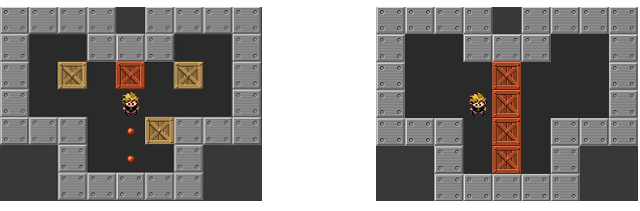
\includegraphics[width=12cm,scale=0.5]{images/sokoban_star_end}
\end{center}
\caption{Sokoban with four blocks solved. Aymeric du Peloux, (\citeyear{sokoban2010})}\label{fig:img_sokoban_solved}
\end{figure}

The solution shown in Figure \ref{fig:img_sokoban_solved} is to use the agent to push blocks located in the left figure to the goal distribution of blocks in the right figure.

\bigskip

In the next Chapter, we will introduce the meta-reasoning proposed for selecting heuristics.

\clearpage